\chapter{Clustering}


% ---------- Mutual Info Score ----------
\clearpage
\thispagestyle{clusteringstyle}
\section{Mutual Info Score}
\subsection{Mutual Info Score}

The Mutual Information (MI) Score can be used to quantify the amount of information shared between two clustering assignments.
It's also particularly useful for comparing the similarity between ground-truth labels and predicted clustering labels.

% Formula
\begin{center}
    FORMULA GOES HERE
\end{center}

The MI score ranges from 0 to +infinity, where 0 indicates no mutual information and higher values signify greater
similarity. To address certain limitations of the standard MI score, such as lack of normalization and agreement by chance, variations like the
Normalized Mutual Information (NMI) score and the Adjusted Mutual Information (AMI) score were developed.

NMI ranges from 0 to 1, while AMI ranges from -1 to 1. The key difference between AMI and NMI is that AMI adjusts for chance. 
AMI equals 0 when the clustering assignments are no more similar than would be expected by chance.

\textbf{When to use Mutual Info Scores?}

Use MI you need a basic measure of shared information between two clusterings. NMI when comparing clustering results with different numbers of
clusters, as it normalizes the score to a standard range. AMI when you want to account for chance.

\coloredboxes{
    \item Symmetric. Switching true label with predicted ones will return the same score.
    \item Lower and upper bounded in the case of the NMI and AMI variations.
    \item Can be used as a consensus score.
}
{
    \item Requires knowledge of ground truth classes.
    \item A permutation of the cluster label values doesn't change the score value in any way. eg. IM([0, 0, 1], [0, 0, 1]) = IM([0, 0, 1], [1, 0, 0])

}

% ---------- rand index ----------
\clearpage
\thispagestyle{clusteringstyle}
\section{Rand Index}
\subsection{Rand Index}

The Rand Index (RI) is a clustering metric that measures the similarity between two clusterings using the predicted labels generated by an algorithm
and the true labels or labels comming from a reference clustering.

\begin{center}
    % Formula of the type:
    % Number of agreeing pairs / Number of pairs
    FORMULA GOES HERE
\end{center}

The standard RI ranges from 0 to 1, where 1 indicates perfect agreement between the predicted and reference clusterings.
However, for random labelings, the RI does not yield values close to 0, as it lacks an adjustment for chance. To address this,
the Adjusted Rand Index (ARI) refines the RI by accounting for randomness. ARI values range from -0.5 to 1, where scores near 0
signify clustering results comparable to random labelings. RI is also equivalent to the accuracy score in a pairwise binary
classification task, evaluating the fraction of pairs correctly classified as "same cluster" (True Positives) or
"different cluster" (True Negatives).


\textbf{When to use Random Index Scores?}

Use RI/ARI when ground truth labels are available for benchmarking clustering performance. A comparison of consensus across
multiple clusterings is needed. Interpretability and connection to pairwise agreement are desired.

\coloredboxes{
    \item Symmetric. Switching true label with predicted ones will return the same score.
    \item Lower and upper bounded ranges for both RI and ARI.
    \item Can be used as a consensus score.
}
{
    \item Requires knowledge of ground truth classes.
    \item Similar to accuracy in binary classification, unadjusted RI is affected by class imbalance, which can result in high 
    RI scores even when the clusterings are significantly different.
}

% ---------- calinski harabasz index ----------
\clearpage
\thispagestyle{clusteringstyle}
\section{CH Index}
\subsection{Calinski Harabasz Index}

The Calinski–Harabasz Index (CH Index), also known as the Variance Ratio Criterion, is a clustering evaluation metric that does
not require ground-truth labels. It measures the quality of clustering by comparing the dispersion between clusters to the
dispersion within clusters.

\begin{center}
    FORMULA GOES HERE
\end{center}

The CH Index is defined as the ratio of the between-clusters dispersion (BCSS) to the within-cluster dispersion (WCSS),
normalized by their respective degrees of freedom. We normalize BCSS and WCSS by their degrees of freedom to ensure comparability
across different values of $k$, avoiding artificial inflation of the score for higher cluster counts.

\textbf{When to use Calinski-Harabasz Index?}

Use CH Index when no ground-truth labels are available to validate the clustering quality. It can also be used to identify the
optimal number of clusters by maximizing the CH Index across different cluster counts.

\coloredboxes{
    \item The CH Index does not rely on labeled data.
    \item The use of degrees of freedom normalization ensures fair comparison across varying $k$ and sample sizes.
}
{
    \item The calculation assumes a Euclidean distance metric, which may limit its applicability for non-Euclidean data.
}

% ---------- contingency matrix ----------
\clearpage
\thispagestyle{clusteringstyle}
\section{Contingency Matrix}
\subsection{Contingency Matrix}

The Contingency Matrix is a tool for evaluating clustering performance by comparing the alignment of predicted cluster
assignments with ground-truth labels. It provides a detailed overview of how well the clusters correspond to the known
categories by counting overlaps between the two.

For a dataset of size $n$, let $k$ be the number of clusters and $C$ the number of ground-truth categories.
The Contingency Matrix is constructed such that the element at position  $(i,j)$ represents the number of data points that belong
to cluster $i$ and category $j$. If this sounds familiar to a Confusion Matrix, it is because it is. In fact, a Confusion Matrix
is a special case of a Contingency Matrix, where the matrix is square, and instead of clusters, we have classes.

\textbf{When to use a Contingency Matrix?}

The contingency matrix is particularly useful when ground-truth labels are available. When you want to analyze how well the
clustering results correspond to the known categories, especially for imbalanced datasets. Or when a deeper understanding
of misclassifications or overlaps between clusters and categories is needed. It most effective when combined with
complementary evaluation methods.

\coloredboxes{
    \item Provides a granular view of the correspondence between clusters and ground-truth categories,
    including misclassifications.
    \item Serves as a basis for other clustering evaluation metrics like Normalized Mutual Information (NMI) or
    Adjusted Rand Index (ARI).
}
{
    \item Requires ground-truth labels.
    \item For datasets with many clusters or categories, the matrix can become large and harder to interpret.
    \item Does not provide a single score.
}

% ---------- pair confusion matrix ----------
\clearpage
\thispagestyle{clusteringstyle}
\section{Pair Confusion Matrix}
\subsection{Pair Confusion Matrix}

The Pair Confusion Matrix is a clustering evaluation metric used to assess the similarity between two clusterings by
comparing pairwise relationships between data points. It is a $2x2$ matrix that extends the idea of the confusion matrix
to clustering scenarios, focusing on whether pairs of points are grouped together or not.

\begin{center}
    MATRIX GOES HERE
\end{center}

It has four key components, each representing a count of point pairs in specific configurations across two clusterings. It can
also be showen that $C_{00} + C_{11} + C_{10} + C_{01} = \frac{n(n-1)}{2}$

\textbf{When to use the Pair Confusion Matrix?}

Use the Pair Confusion Matrix when evaluating clustering algorithms that produce hard cluster assignments and when ground truth
is available.

\coloredboxes{
    \item Breaks down clustering agreements and disagreements into familiar components (TP, TN, FP, FN).
}
{
    \item Requires ground-truth labels.    
    \item Computation can be slow for large datasets due to the pairwise comparison of all points.
    \item Does not provide a single score.
}

\clearpage

\thispagestyle{customstyle}

Analyse the following example to understand how to build the matrix. Lets say we have the following clustering results.

\[
\begin{array}{l|cccccc}
    & \text{$obj_{1}$} & \text{$obj_{2}$} & \text{$obj_{3}$} & \text{$obj_{4}$} \\
\hline
\text{True Labels} & 0 & 0 & 1 & 0 \\
\text{Pred Labels} & 0 & 1 & 0 & 1 \\
\end{array}
\]

With this we can compute $C_{00}$, $C_{11}$, $C_{10}$ and $C_{01}$.

\begin{itemize}
    \item $C_{00}$: number of pairs with different true and pred labels = $(obj_{2}, obj_{3})$; $(obj_{3}, obj_{4})$; $(obj_{3}, obj_{2})$; $(obj_{4}, obj_{3})$ = $4$
    \item $C_{11}$: number of pairs with same true and pred labels = $(obj_{2}, obj_{4})$; $(obj_{4}, obj_{2})$ = $2$
    \item $C_{10}$: number of pairs with same true but different pred labels = $(obj_{1}, obj_{2})$; $(obj_{1}, obj_{4})$;
    $(obj_{2}, obj_{1})$; $(obj_{4}, obj_{1})$ = $4$
    \item $C_{01}$: number of pairs with different true but same pred labels = $(obj_{1}, obj_{3})$; $(obj_{3}, obj_{1})$ = $2$
\end{itemize}

Thus, the final Pair Confusion Matrix looks like:
\begin{center}
    \[
        C =
        \begin{bmatrix}
            4 & 2 \\
            4 & 2
        \end{bmatrix}
    \]
\end{center}

\orangebox{Did you know that...}
{MISSING FUN FACT}


\textbf{Other related metrics}

% ---------- Completeness Score ----------
\clearpage
\thispagestyle{clusteringstyle}
\section{Completeness Score}
\subsection{Completeness Score}

The Completeness Score evaluates the degree to which members of a ground-truth class are assigned to the same cluster in a
clustering solution. It is one of two complementary measures (the other being Homogeneity Score) used to assess the quality of
clustering. Completeness is mathematically defined using conditional entropy between cluster labels and assignments.

% \[
% \text{Completeness} = 1 - \frac{H(K \mid C)}{H(K)}
% \]

\begin{center}
    FORMULA GOES HERE
\end{center}

A perfect completeness score of 1 indicates that all members of a single class are contained within a single cluster. 
A score of 0 means the clustering completely fails to keep members of the same class together.

\textbf{When to use the Completeness Score?}

The Completeness Score is particularly useful when you need to evaluate how well a clustering algorithm preserves class membership
within individual clusters. It is commonly applied in scenarios such as document clustering, where documents belonging to the same
topic should ideally belong to one cluster.

\coloredboxes{
    \item Class-Focused Evaluation. Completeness measures how well class integrity is preserved in clustering,
    providing a clear diagnostic for one aspect of clustering quality.
    \item Lower and upper bounded.
    \item Clustering algorithm agnostic.
}
{
    \item Requires ground-truth labels.
    \item Trade-Off with Homogeneity. Completeness tends to decrease as completeness increases, creating a challenge when
    trying to optimize both simultaneously.
    \item Not normalized with regards to random labeling.
}

\clearpage

\thispagestyle{customstyle}

\textbf{Other related metrics}

The Completeness Score is best used in conjunction with the Homogeneity Score or V-Measure. While completeness focuses on
ensuring all members of a class are in the same cluster, homogeneity ensures that clusters do not mix members from different
classes. V-Measure provides a balanced harmonic mean of these two metrics, offering a single comprehensive evaluation of
clustering quality​.

% ---------- Homogeneity Score ----------
\clearpage
\thispagestyle{clusteringstyle}
\section{Homogeneity Score}
\subsection{Homogeneity Score}

The Homogeneity Score measures how well each cluster contains only data points from a single ground-truth class.
It is designed to assess the purity of clusters by evaluating the entropy of class distributions within each cluster.

\begin{center}
    FORMULA GOES HERE
\end{center}

A score of 1.0 indicates perfect homogeneity, meaning every cluster contains data points from only one class. 
A score of 0.0 indicates that the class distribution within clusters mirrors the overall dataset distribution,
showing no class distinction within clusters.

\textbf{When to use the Homogeneity Score?}

The Homogeneity Score is particularly valuable when evaluating the ability of a clustering algorithm to form well-defined,
class-pure clusters. Common applications include customer segmentation, where customers within a cluster should share similar characteristics.
Topic modeling, where documents within a cluster should belong to the same topic.

\coloredboxes{
    \item Cluster Purity Focus. Homogeneity emphasizes the purity of clusters, providing a clear diagnostic of whether
    clusters contain mixed classes.
    \item Lower and upper bounded.
    \item Clustering algorithm agnostic.
}
{
    \item Requires ground-truth labels.
    \item Trade-Off with Completeness. Homogeneity tends to decrease as completeness increases, creating a challenge when trying to optimize both simultaneously.
    \item Not normalized with regards to random labeling.
}


\clearpage

\thispagestyle{customstyle}

\textbf{Other related metrics}

Homogeneity is best used alongside Completeness or V-Measure. While Homogeneity ensures clusters are internally consistent with
respect to class membership, Completeness ensures that all members of a class are grouped together. V-Measure combines the two
into a single harmonic mean, providing a balanced evaluation of clustering quality

% ---------- V Measure ----------
\clearpage
\thispagestyle{clusteringstyle}
\section{V Measure}
\subsection{V Measure}

V-Measure is an external clustering evaluation metric that combines the strengths of two complementary criteria: Homogeneity
(how pure clusters are with respect to ground-truth classes) and Completeness (how well all members of a class are grouped into
the same cluster). It is computed as the harmonic mean of these two scores, similar to how precision and recall are combined into
the F-score.

\begin{center}
    FORMULA GOES HERE
\end{center}

By design, V-Measure is bounded between 0.0 and 1.0, with higher scores indicating better clustering quality. A score of 1.0
means that both homogeneity and completeness are perfectly satisfied.

\textbf{When to use the V-measure?}

V-Measure is ideal for evaluating clustering solutions when you need a balanced assessment of both purity within clusters and the
completeness of class representation.

\coloredboxes{
    \item Combines homogeneity and completeness into a single score, providing a holistic evaluation of clustering quality.
    \item The $\beta$ parameter allows customization to prioritize either homogeneity or completeness based on specific use cases.
    \item Clustering algorithm agnostic.
}
{
    \item Requires ground-truth labels.
    \item V-Measure inherits the trade-off between homogeneity and completeness. Adjusting one often impacts the other, making it
    challenging to optimize both in some scenarios.
    \item Not normalized with regards to random labeling.
}

\clearpage

\thispagestyle{customstyle}

\textbf{Other related metrics}

V-Measure excels as a comprehensive metric for clustering evaluation. However, for specific insights, it can be supplemented with
individual Homogeneity and Completeness scores. Additionally, pair-based measures like Adjusted Rand Index (ARI) or
information-theoretic measures like Variation of Information (VI) may provide complementary perspectives in specific use cases​.

% ---------- Davis Bouldin Score ----------
\clearpage
\thispagestyle{clusteringstyle}
\section{Davis Bouldin Score}
\subsection{Davis Bouldin Score}

% ---------- Fowlkes Mallows Score ----------
\clearpage
\thispagestyle{clusteringstyle}
\section{Fowlkes Mallows Score}
\subsection{Fowlkes Mallows Score}

% ---------- Silhouette Score ----------
\clearpage
\thispagestyle{clusteringstyle}
\section{Silhouette Score}
\subsection{Silhouette Score}

The Silhouette Coefficient measures how well a data point fits within its assigned cluster compared to other clusters. 
It quantifies how similar a sample is to its own cluster (cohesion) compared to the nearest neighboring cluster (separation).
The Silhouette Coefficient $s(i)$ for a given data point $i$ in the cluster $C_I$, where $|C_I|$ is the number of data points in $C_I$, is given by:

\begin{center}
\tikz{
\node[inner sep=2pt, font=\Large] (a) {
{
$\displaystyle
s(i) = 
\begin{cases}
\frac{{\color{cyan}b(i)} - {\color{nmlpurple}a(i)}}{max\left\{ {\color{nmlpurple}a(i)}, {\color{cyan}b(i)} \right\}}  & if\, |C_I| > 1 \\
0  & if\, |C_I| = 1
\end{cases}
$
}
};
\draw[-latex,cyan, semithick] ($(a.north)+(-0.9,0.05)$) to[bend right=15] node[pos=1, left] {measures cohesion} +(-1,.5); 
\draw[-latex,nmlpurple, semithick] ($(a.north)+(0.2,0.05)$) to[bend left=15] node[pos=1, right] {measures separation} +(1,.5); 
% \draw[-latex,nmlpurple, semithick] ($(b.north)+(0.1,0.05)$) to[bend left=15] node[pos=1, left] {True negatives} +(-1,-.5); 
}
\end{center}

Where  $a(i)$ is the mean distance between a sample and all other points in the same cluster (mean intra-cluster distance), 
and  $b(i)$ is the mean distance between a sample and all points in the nearest different cluster (mean nearest-cluster distance). 
The value of  $s(i)$ lies between -$1$ and  $1$, where  $s(i) \approx 1$ indicates that the data point is well-clustered, 
 $s(i) \approx 0$ means the data point is on or very close to the boundary between two clusters, and  $s(i) \approx -1$ 
suggests that the data point has been misclassified into the wrong cluster.

\textbf{When to use Silhouette Score?}

Use Silhouette Score when the ground truth labels are unknown and the evaluation must be performed using the model itself.

\coloredboxes{
\item It provides a clear and intuitive measure of how well clusters are separated, +1 highly dense and -1 for incorrect clustering.
}
{
\item Silhouette Score can generally be higher for convex clusters than other clusters, such as density based clusters.
\item Higher Silhouette Score doesn't necessarily indicate that the clusters will have equal sizes; the clusters can still vary in cardinality. 
}

% ----------  Consensus Score ----------
\clearpage
\thispagestyle{clusteringstyle}
\section{ Consensus Score}
\subsection{ Consensus Score}


% ----------  Dunn Index ----------
\clearpage
\thispagestyle{clusteringstyle}
\section{ Dunn Index}

% Define colors
\definecolor{nmlpurple}{RGB}{128,0,128}

The Dunn Index is used to evaluate the quality of clusters by measuring both the separation between the clusters and compactness within clusters. It considers the smallest distance between points in different clusters (inter-cluster distance) and the largest distance within a single cluster (intra-cluster distance) to evaluate how well-defined the clusters are. A higher Dunn Index indicates that the clustering configuration has well-separated and compact clusters, while a lower Dunn Index suggests poor separation or high dispersion within clusters.\\

The Dunn Index for a given clustering solution with \( k \) clusters \( C_1, C_2, \ldots, C_k \) is defined as:

\begin{center}
	\begin{tikzpicture}
		\node[inner sep=2pt, font=\Large] (a) {
			$\displaystyle
			D = \frac{\min\limits_{1 \leq i < j \leq k} \{ \text{dist}(C_i, C_j) \}}{\max\limits_{1 \leq i \leq k} \{ \text{diam}(C_i) \}}
			$
		};
		\draw[-latex, cyan, semithick] ($(a.north east)+(0.2,-0.1)$) to[bend left=15] node[pos=1, right] {measures inter-cluster distance} +(2,0.5); 
		\draw[-latex, nmlpurple, semithick] ($(a.south east)+(0.2,0.1)$) to[bend right=15] node[pos=1, right] {measures intra-cluster distance} +(2,-0.5); 
	\end{tikzpicture}
\end{center}

where:
\begin{itemize}
	\item \(\text{dist}(C_i, C_j)\) represents the distance between clusters \( C_i \) and \( C_j \), often calculated as the minimum distance between any two points in different clusters (inter-cluster distance).
	\item \(\text{diam}(C_i)\) represents the diameter of cluster \( C_i \), typically defined as the maximum distance between any two points within the same cluster (intra-cluster distance).
\end{itemize}

\textit{The Dunn Index ranges from 0 to infinity, with higher values indicating better-defined clusters. Values closer to 0 suggest that clusters are either overlapping or not sufficiently compact.}\\

\textbf{When to Use Dunn Index?}

The Dunn Index is primarily used when evaluating clustering results in applications where the structure and separation of clusters are critical. It is useful in determining whether a clustering algorithm has successfully created distinct, dense clusters without overlap. The Dunn Index is particularly valuable for comparing clustering algorithms, such as K-means, hierarchical clustering, and DBSCAN, especially when the number of clusters is uncertain, or various configurations need to be tested.

% strength and weakness box
\coloredboxes{
	\item Considers both intra-cluster compactness and inter-cluster separation.
	\item Useful for determining the best number of clusters.
	\item Higher values indicate better-defined clusters.
	\item Helps compare clustering algorithms.
}
{
	\item Outliers can reduce the Dunn Index value, affecting accuracy.
	\item High resource use for large datasets.
	\item Less effective for irregular shapes.
	\item Sensitive to unnormalized features.
	\item Can be unreliable in high-dimensional spaces.
}

% Inserting the image
\begin{figure}[h!]
	\centering
	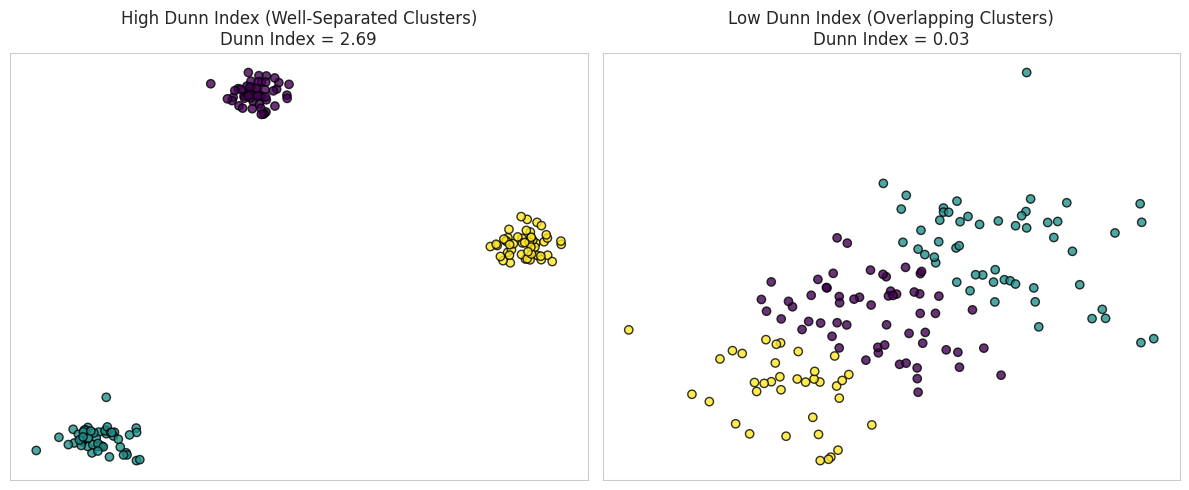
\includegraphics[width=\textwidth]{/figures/Dunn_Index_Visualized.png} 
	\caption{Illustration of High and Low Dunn Index Values}
\end{figure}

% Adding the explanation below the image
\textbf{In the visualization above:}
\begin{itemize}
	\item \textbf{Left Plot (High Dunn Index):} This example illustrates clusters that are well-separated and compact. Each cluster (shown in blue, green, and purple) is distinct, with clear boundaries and minimal overlap with other clusters. The points within each cluster are closely packed, which leads to a small maximum intra-cluster distance (diameter). Furthermore, the minimum distance between clusters (inter-cluster distance) is large, reinforcing the separation between clusters. These characteristics yield a high Dunn Index, signifying a high-quality clustering configuration where clusters are well-defined and do not overlap.
	\item \textbf{Right Plot (Low Dunn Index):} This example illustrates clusters that are overlapping and dispersed. The clusters lack distinct boundaries, and points from different clusters are intermixed. The large maximum intra-cluster distance, due to dispersed points within clusters, combined with a small minimum inter-cluster distance, because of overlapping clusters, results in a low Dunn Index. This clustering configuration suggests poor clustering quality, as the clusters are not compact or well-separated.
\end{itemize}

\subsection{ Dunn Index}

